% Chapter Template

\chapter{Kernel-Based Structured Output Learning} % Main chapter title
\label{Chapter4} % Change X to a consecutive number; for referencing this chapter elsewhere, use \ref{ChapterX}
\lhead{Chapter 4. \emph{Kernel-Based Structured Output Learning}} % Change X to a consecutive number; this is for the header on each page - perhaps a shortened title

\rule{\textwidth}{0.4pt} \\[0.5cm]
\textit{``Nothing is more practical than a good theory."}

\begin{flushright}
Vladimir Vapnik
\end{flushright}
\rule{\textwidth}{0.4pt} 

In previous two chapters, structured data are encoded and manipulated within graphs. This chapter, by contrast, 
deals with structures with \emph{kernel methods}. The kernel methods have been incorporated with many classic data analysis 
techniques and enable them to detect nonlinear patterns in 
data \citep{citeulike:Taylor_Nello_Kernel}.   
Meanwhile, here another function of kernels is more exploited: a kernel is designed as a similarity function on a pair of instances by  
considering the inter-dependency among the elements in each instance. This property is usually ignored when people use kernels.   
For instance, a degree-2 polynomial kernel defined on $\mathbf{x}\in\mathbb{R}^d$ is:
\begin{equation}
    K(\mathbf{x}^{(i)},\mathbf{x}^{(j)})=\left(\langle \mathbf{x}^{(i)},\mathbf{x}^{(j)} \rangle +c\right)^2
\label{equ:pol_kernel}
\end{equation}
where $c$ is a constant, $\mathbf{x}^{(i)},\mathbf{x}^{(j)}$ are two instances. The feature map induced by the kernel is:      
\begin{equation}
    \phi(\mathbf{x})=[x_d^2,\cdots,x_1^2, \sqrt{2}x_d x_{d-1}, \cdots, \sqrt{2}x_2 x_{1}, \sqrt{2c}x_d,\cdots, \sqrt{2c}x_1,c]^\top 
     \label{equ:pol_feature_map}
\end{equation}
It can be seen that the interactions between every pair of elements ($x_d, x_{d-1}$) are encoded in $\phi(\mathbf{x})$, which is 
more informative than treating elements independently when no kernel is applied.  
The pairwise interactions within $\phi(\mathbf{x})$ are analogous to the pairwise edges in graphical models. However, kernel methods can go beyond graphical models by providing 
higher-order interactions, \emph{e.g.} degree-3 polynomial can capture dependencies within triplets.  

Kernels were usually used on inputs since the output is a single scalar value in classic classification and regression tasks.   
When outputs are structured in modern data analysis, it is interesting to try adding kernels also on outputs.     
This chapter provides two attempts on structured-outputs-kernels. 
More concretely, two novel methods are proposed for multi-label learning: \emph{joint SVM} and \emph{kernel generalized homogeneity analysis} (KGHA). 
These two methods are presented in section \ref{sec:joint_SVM} and section \ref{sec:KGHA} respectively. In particular, the joint SVM is closely related to 
the \emph{structural SVM}, which is reviewed in subsection \ref{subsec:SSVM}. KGHA, on the other hand, is an extension of \emph{homogeneity analysis}, which is 
a popular multivariate analysis technique. Section \ref{sec:homo} presents an application of homogeneity analysis on object-action learning.    




%----------------------------------------------------------------------------------------
%	SECTION 1
%----------------------------------------------------------------------------------------

\section{Joint SVM}
\label{sec:joint_SVM}

%-----------------------------------
%	SUBSECTION 1
%-----------------------------------
\subsection{Structural SVM for Multi-Label Learning}
\label{subsec:SSVM}
This subsection introduces structural SVM \citep{StructSVM} based on standard SVM and studies its application 
in multi-label learning. Structural SVMs can also be considered as max-margin Markov networks (M$^3$Ns), which was studied in subsection \ref{subsec:MMMN}. 
Standard SVM is a binary classifier, which has been well 
understand and widely used in many applications.  
Its two advantageous components are \emph{maximum margins} and \emph{input kernels}. 
The maximum-margin principle is a reflection of statistical learning theory \citep{Vapnik} on 
linear binary classification. 
Kernels provide powerful mechanisms enabling the linear classifier to separate highly non-linear data. 
The critical observation of kernel methods is that a kernel function can be defined on a pair of data 
instances to implicitly map them to a \emph{reproducing kernel Hilbert space} (RKHS):   
\begin{equation}
    K_\phi(\mathbf{x}^{(i)},\mathbf{x}^{(j)})=\langle \phi(\mathbf{x}^{(i)}),\phi(\mathbf{x}^{(j)}) \rangle
 \label{equ:kernel_trick}
\end{equation}
where $\mathbf{x}^{(i)}, \mathbf{x}^{(j)}\in\mathbb{R}^d$ are two input training instances, $\phi$ is the feature map induced by kernel function $K_\phi$, and $\phi(\mathbf{x}^{(i)})$ is the 
representation of 
$\mathbf{x}^{(i)}$ in the RKHS $\mathcal{H}_\phi$.
Given the training dataset $\{\mathbf{x}^{(i)}\in\mathbb{R}^d,y^{(i)}\in\{+1,-1\}\}_{i=1}^m$, the primal form of training SVM is:
\begin{equation}
\begin{array}{rl} 
    \displaystyle \arg\min_{ \mathbf{w} \in \mathbb{R}^{\mathcal{H_{\phi}}}}   & \frac{1}{2} ||\mathbf{w}||^2+C\sum_{i=1}^m \xi^{(i)} \\
    \text{s.t.} & y^{(i)} \left(\mathbf{w}^\top \phi (\mathbf{x}^{(i)})\right) \geq 1-\xi^{(i)}, \xi^{(i)} \geq 0,  i\in \{1,\dots,m\}
\end{array}
\label{equ:hard_svm}
\end{equation}
where $\mathbf{w}$ is a linear hyperplane in $\mathcal{H}_\phi$, $\xi^{(i)}$ are slack variables for the tolerance of noise, and $C$ is a trade-off parameter. 
The diagram in Figure \ref{fig:SVM} illustrates basic characteristics of SVM.   
(\ref{equ:hard_svm}) differs from usual SVM formulation slightly at the absence of a bias term. Here we ignore the bias since 
it can be absorbed in $\mathbf{w}$. 
\footnote{When a Polynomial kernel is used, a bias term is already in its corresponding feature map. When a Gaussian kernel is used, an input vector can be 
augmented with one extra constant.}


\begin{figure}[t]
	\includegraphics[width=\textwidth]{./Figures/SVM_prime}	
	\caption{Understanding the primal form of SVM.}
	\label{fig:SVM}
\end{figure}


Here, to make the transition from SVM to structural SVM more smooth, an alternative interpretaion  
of the primal form of SVM is presented. 
First, denote $y^{(i)} \left(\mathbf{w}^\top \phi (\mathbf{x}^{(i)})\right)$ in the constraints of (\ref{equ:hard_svm}) as a score function $F(\mathbf{x}^{(i)},y^{(i)}; \mathbf{w})$, then  
for binary outputs $y^{(i)}$, $F\left(\mathbf{x}^{(i)},y^{(i)}; \mathbf{w}\right)- F\left(\mathbf{x}^{(i)},-y^{(i)}; \mathbf{w}\right)=2\times F\left(\mathbf{x}^{(i)}),y^{(i)}; \mathbf{w}\right)$. 
Also, a distance function between binary outputs can be denoted by $d(y^{(i)},-y^{(i)})=|y^{(i)}-(-y^{(i)})|=2$. Then by replacing $C$ with $\frac{C}{2}$, (\ref{equ:hard_svm}) can be rewritten 
as:
\begin{equation}
\begin{array}{rl}
\displaystyle \arg\min_{ \mathbf{w} \in \mathbb{R}^{\mathcal{H_{\phi}}}}   & \frac{1}{2} ||\mathbf{w}||^2+C\sum_{i=1}^m \xi^{(i)} \\
                                                                       \text{s.t.} & \forall i, F\left(\mathbf{x}^{(i)},y^{(i)}; \mathbf{w}\right)- F\left(\mathbf{x}^{(i)},-y^{(i)}; \mathbf{w}\right) \geq d(y^{(i)},-y^{(i)})-\xi^{(i)}, \xi^{(i)} \geq 0 
\end{array}
\label{equ:binary_SSVM}
\end{equation}
Structural SVM \citep{StructSVM} is a simple extension of (\ref{equ:binary_SSVM}) by considering more general $y$. 
Assume that the structured output $\mathbf{y}\in\mathcal{Y}$ and $|\mathcal{Y}|$ is more than 
two. Similarly, a score function can be introduced on a pair of input and output based on the 
nature of the task: $F(\mathbf{x},\mathbf{y};\boldsymbol{\theta})$ where $\boldsymbol{\theta}$ is
a parameter set. Then the primal form of the structural SVM can be   
\begin{equation}
\begin{array}{rl}
\displaystyle \arg\min_{ \mathbf{w} \in \mathbb{R}^{\mathcal{H_{\phi}}}}   & \frac{1}{2} ||\mathbf{w}||^2+C\sum_{i=1}^m \xi^{(i)} \\
	\text{s.t.} & \forall i, \forall \mathbf{y}^\prime\in \mathcal{Y}, F\left(\mathbf{x}^{(i)},\mathbf{y}^{(i)}; \mathbf{w}\right)- F\left(\mathbf{x}^{(i)},y^{\prime}; \mathbf{w}\right)\geq d(\mathbf{y}^{(i)},\mathbf{y}^\prime)-\xi^{(i)}, \xi^{(i)} \geq 0 
\end{array}
\label{equ:binary_SSVM}
\end{equation}
which is equivalent to that of a Max-margin Markov network (M$^3$N).     
Structural SVM can be applied on general structured $\mathbf{y}$. In multi-label learning with $L$ labels, $\mathbf{y}$ is a $L-$dimensional binary vector. 
Similarly to M$^3$Ns, solving (\ref{equ:binary_SSVM}) involves exponential number of constraints, and therefore is in general intractable.        

\subsection{Joint SVM: Output Kernel Learning and Regularization }
The joint SVM was developed with a special focus on the interdependencies within outputs in multi-label learning.
Essentially, the joint SVM is equivalent to SSVM with a linear output kernel plus a regularization on the kernel.  
Therefore, a linear kernel on outputs is automatically learned to capture the interdependencies within outputs.  
Furthermore, if prior knowledge about the interdependencies is available, a user-specified output kernel can be 
straightforwardly mounted in Joint SVM as well.  
In both cases, the computation complexity of Joint SVM is almost the same as a single SVM, in contrary to the 
exponential complexity in structural SVM. 
Joint SVM was shown to yield substantial
improvements, in terms of both accuracy and efficiency, over
training them independently. In particular, it outperforms many
other state-of-the-art algorithms according to empirical results
on an image-annotation benchmark database. 

More technique detials and results are presented in the paper I and paper III by the author. 
\begin{shaded}
{\Huge I.} \textbf{Hanchen Xiong}, Sandor Szedmak, Justus Piater. {\it Implicit Learning of Simpler Output Kernels for Multi-Lable Prediction}, NIPS workshop on Representation and Learning Methods for Complex Outputs (NIPS-RLCO2014).  
\vspace{-.2cm}

{\Huge III.} \textbf{Hanchen Xiong}, Sandor Szedmak, Justus Piater. {\it Scalable, Accurate Image Annotation with Joint SVMs and Output Kernels}, Neurocomputing Journal (Accepted).  
\vspace{-.2cm}
\end{shaded}



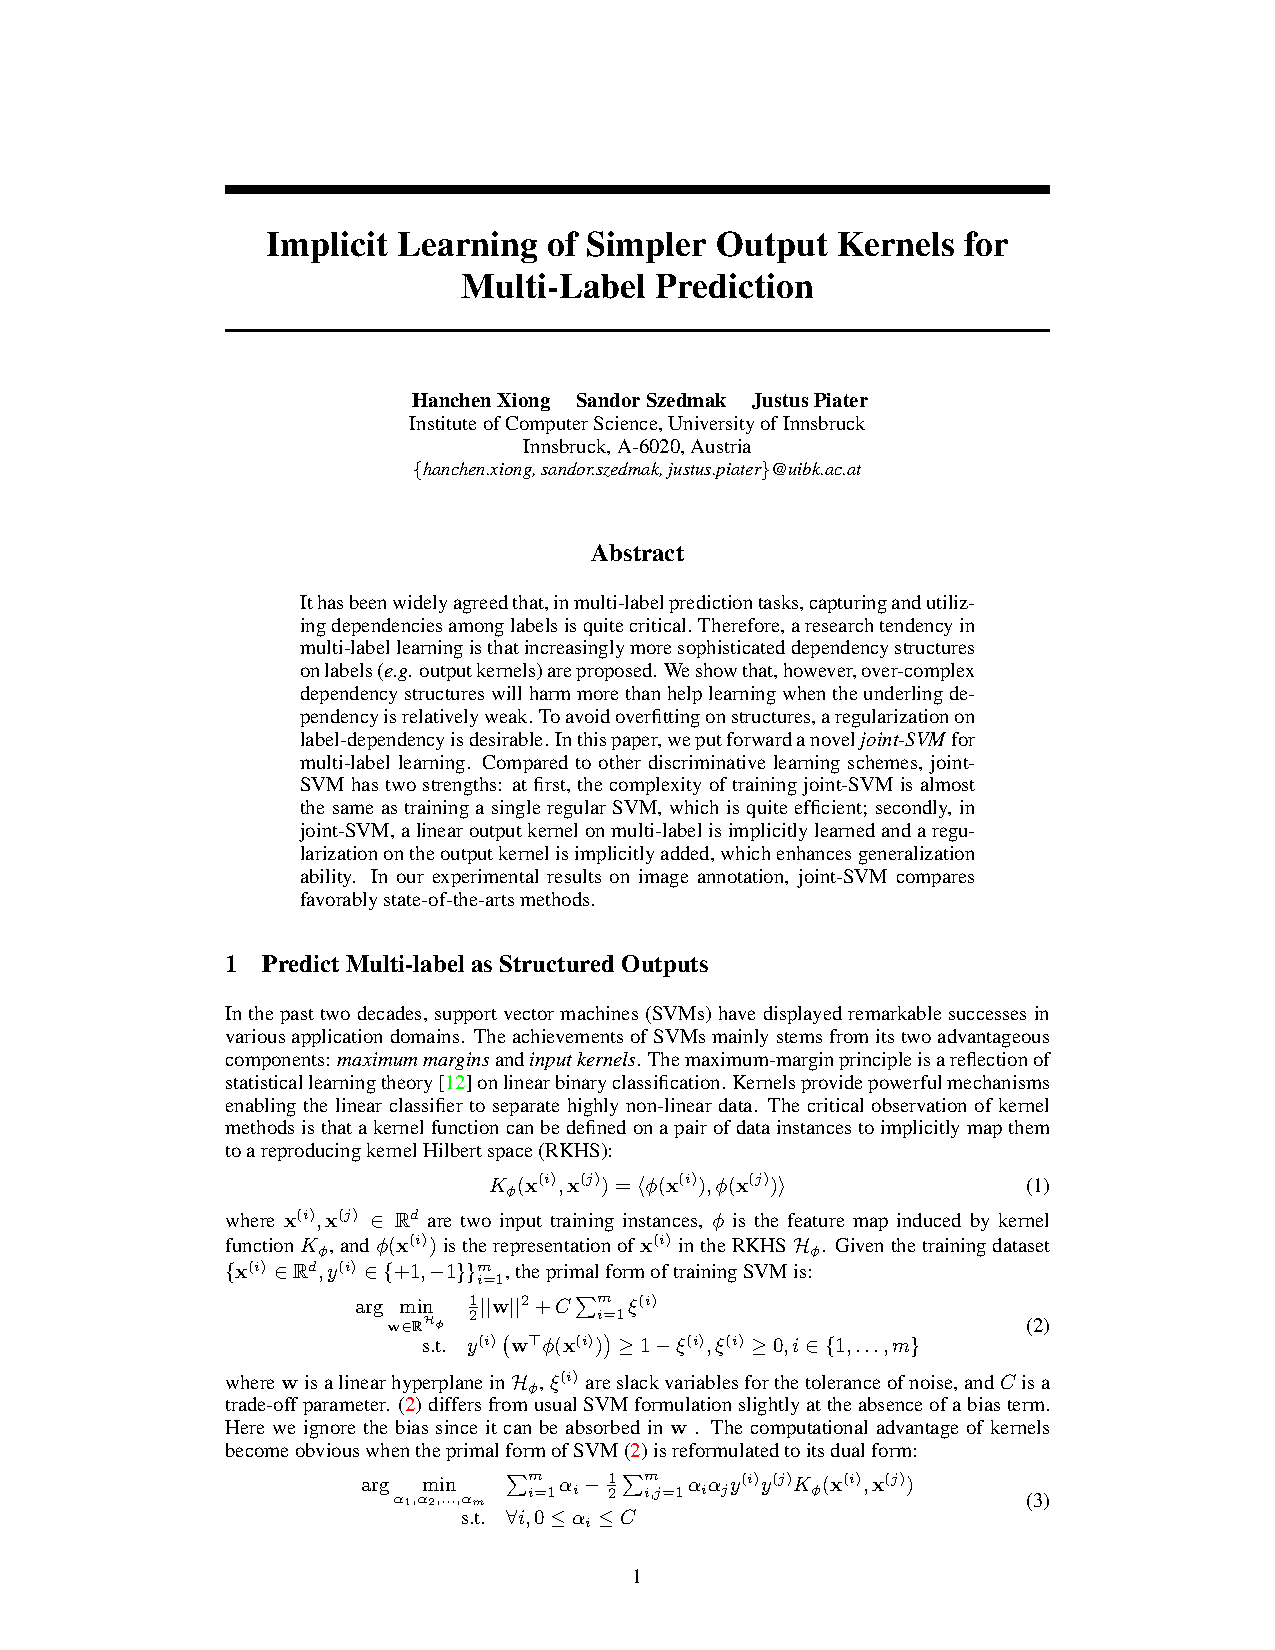
\includepdf[offset=3cm -2cm, scale=1, pages=-,pagecommand={\pagestyle{fancy}}]{./Papers/Xiong-2014-NIPS-RLCO.pdf}
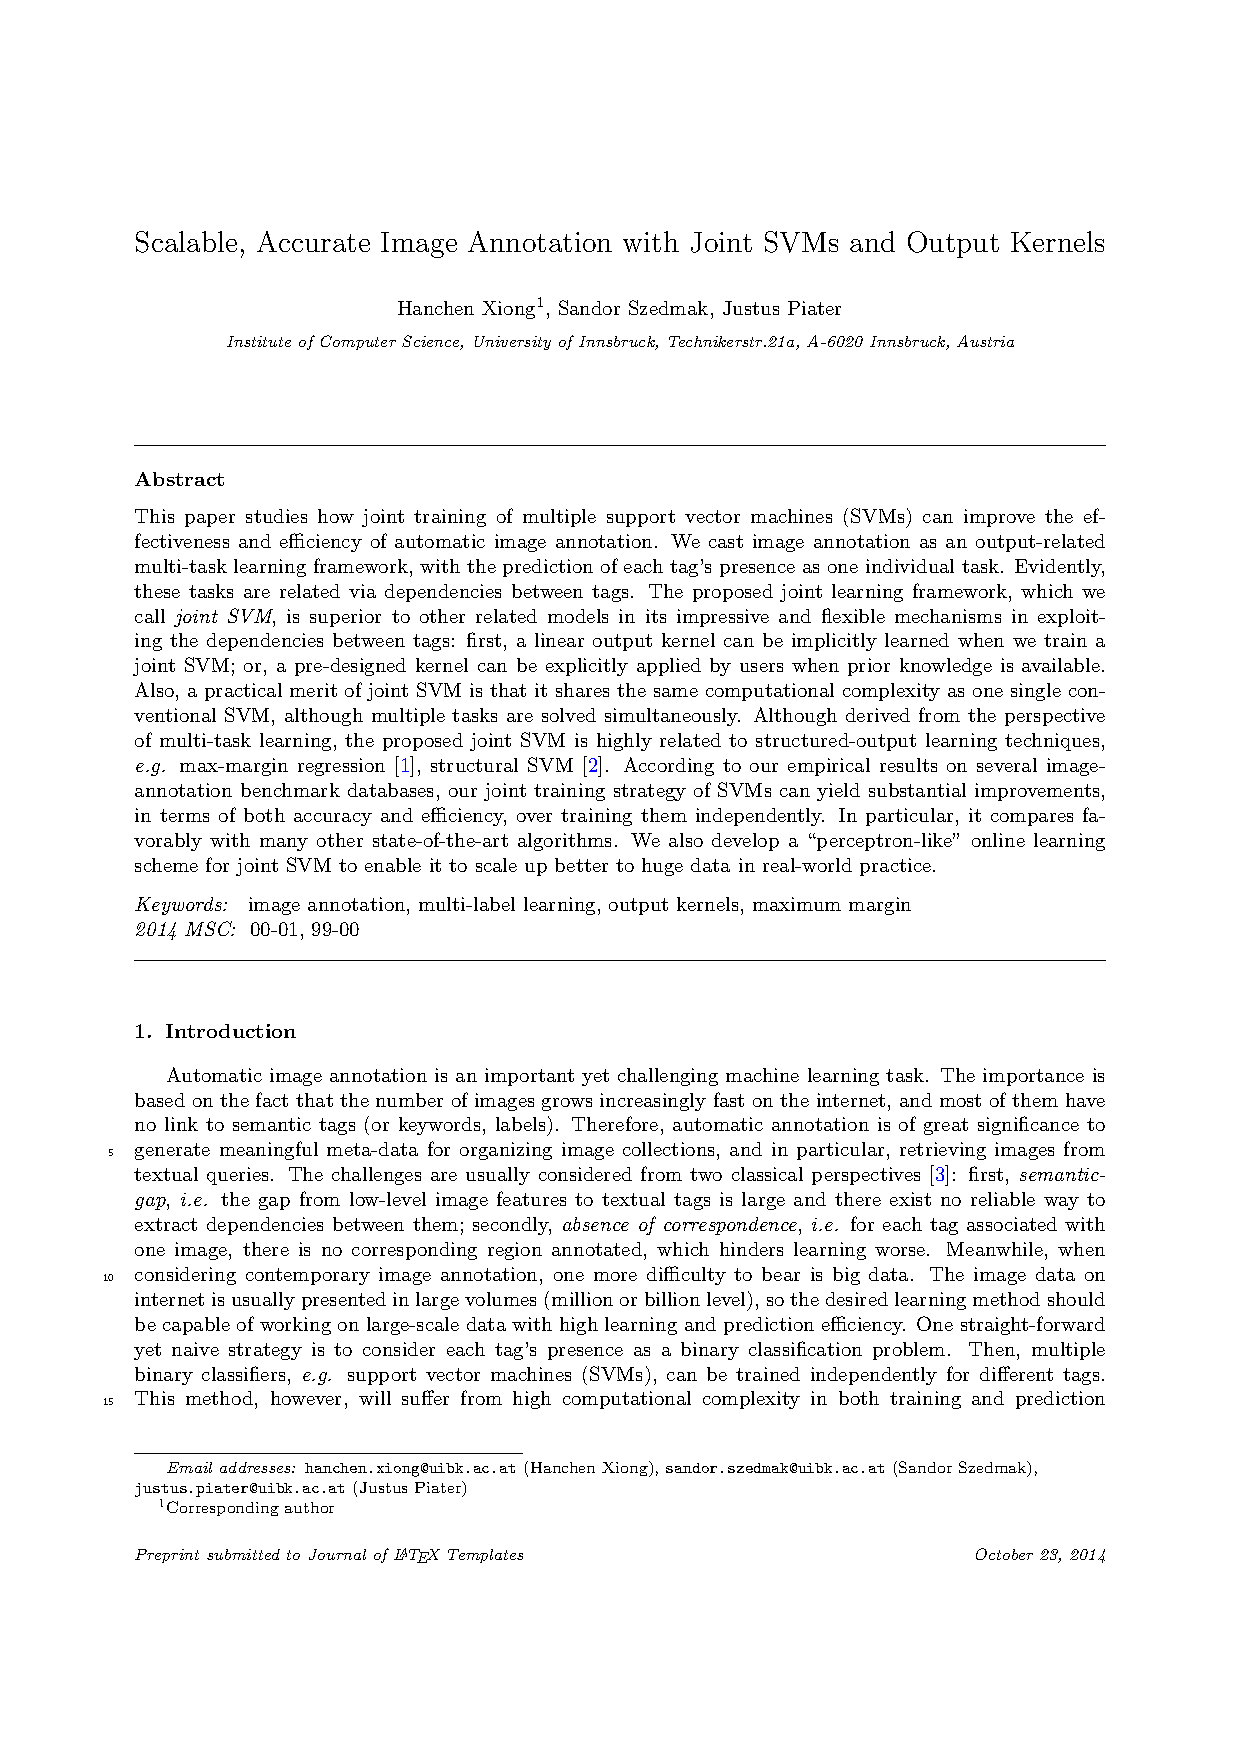
\includepdf[offset=3cm -2cm, scale=1, pages=-,pagecommand={\pagestyle{fancy}}]{./Papers/Xiong-2015-NEUCOM.pdf}





%----------------------------------------------------------------------------------------
%	SECTION 2
%----------------------------------------------------------------------------------------
\section{Homogeneity Analysis for Object-Action Relation Learning}
\label{sec:homo}
In statistics community, structured data are usually handled with \emph{multivariate analysis} (MVA) techniques. For instance,      
\emph{canonical correlation analysis} (CCA) has been used for modeling the dependencies between two set of variables. 
Another case, \emph{homogeneity analysis}, is for multiple categorical values. Both CCA and homogeneity analysis detect
the dependencies among variables by projecting them in low-dimensional spaces. Therefore, these two techniques are also  
often used as \emph{visualization tools} for high-dimensional data.   
Intuitively speaking, MVA techniques model the joint distributions of multiple variables with low-rank projections, in which 
dependencies are implicitly encoded.  


In this section, homogeneity analysis is briefly introduced, and in particular, its application on object-action learning is studied.      
Homogeneity analysis fits the scenario well since the objects' properties and action effects are usually represented by 
categorical values.  More technical details and results are presented in the paper VII by the author. 


\begin{shaded}
{\Huge VII.} \textbf{Hanchen Xiong}, Sandor Szedmak, Justus Piater {\it Homogeneity Analysis for Object-Action Relations Reasoning in Kitchen Scenarios}, 
In Proceedings of 2nd Workshop on Machine Learning for Intelligent Systems (MLIS13), pp 37-44,  2013, ACM. 
\vspace{-.2cm}
\end{shaded}

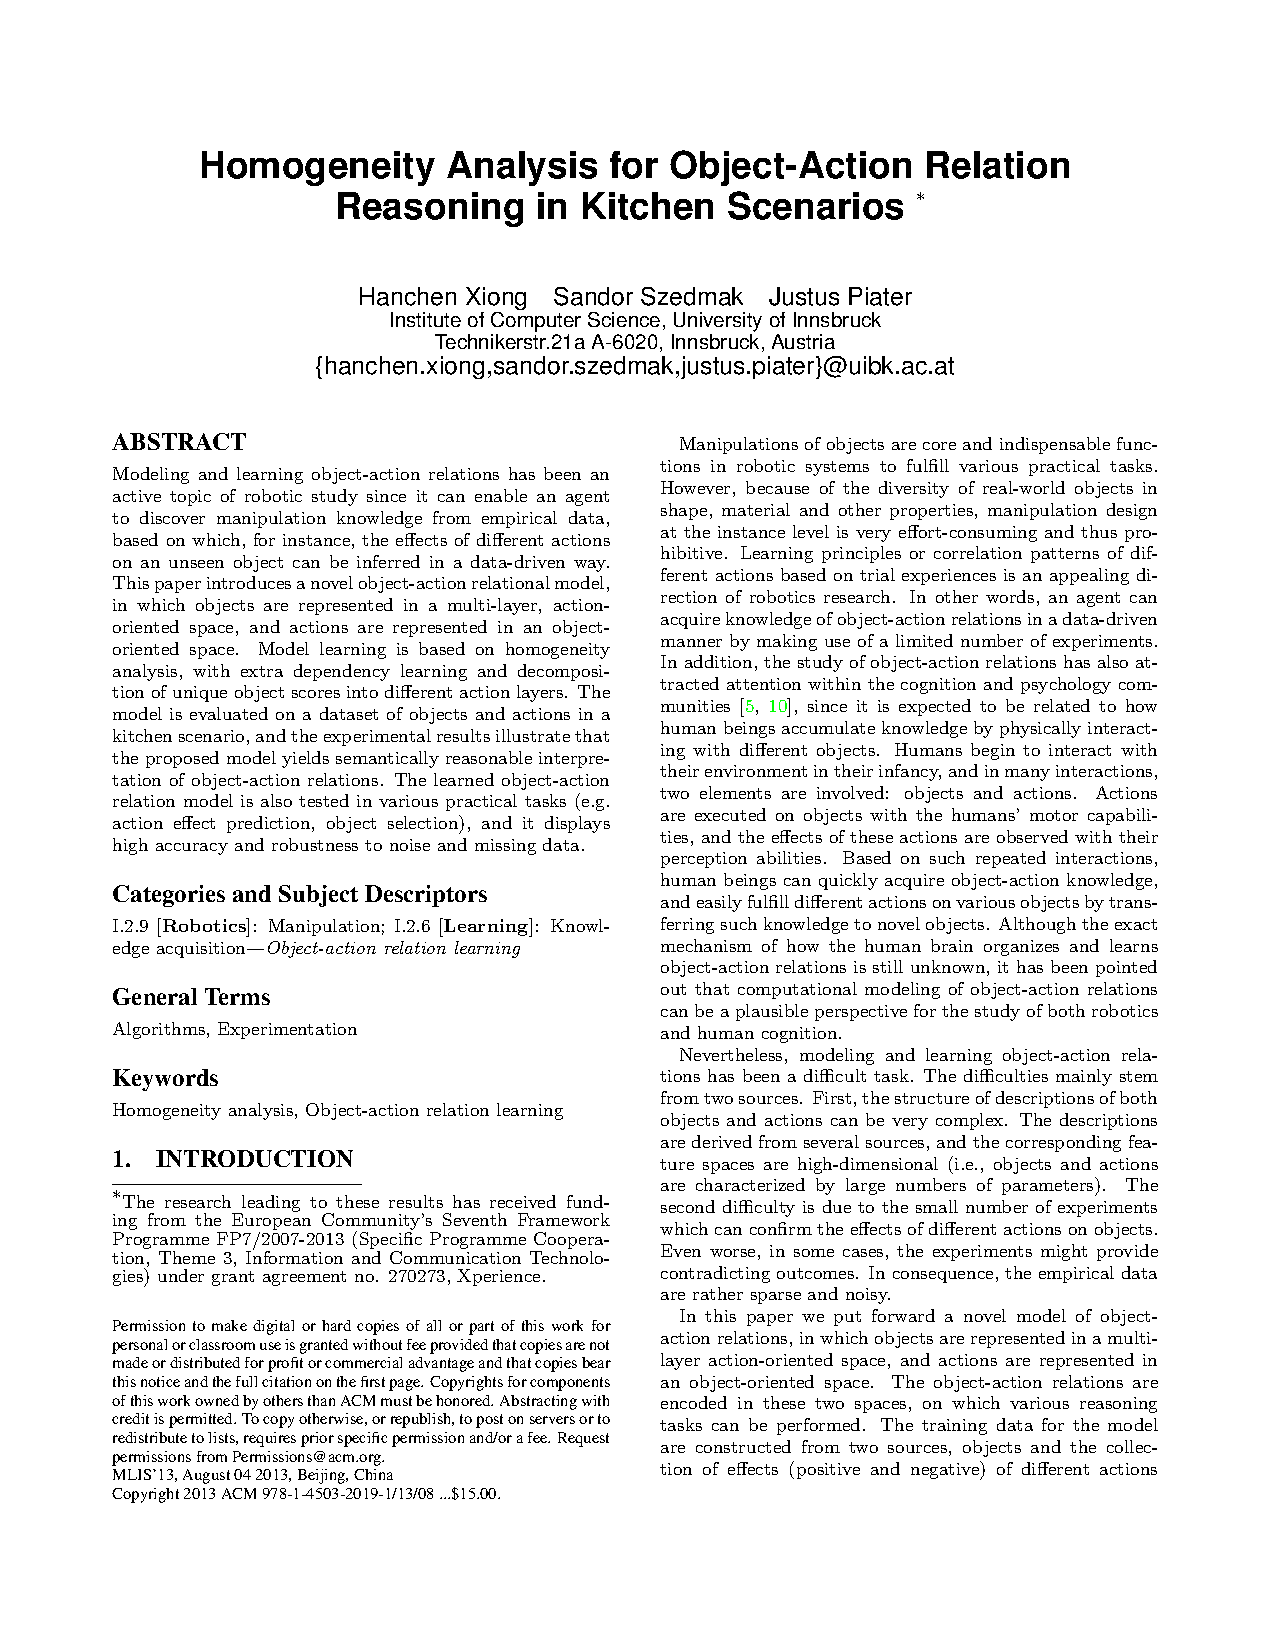
\includepdf[offset=3cm -3cm, scale=1, pages=-,pagecommand={\pagestyle{fancy}}]{./Papers/Xiong-2013-MLIS.pdf}

%----------------------------------------------------------------------------------------
%	SECTION 3
%----------------------------------------------------------------------------------------

\section{Multi-Label Learning with Kernel Generalized Homogeneity Analysis}
\label{sec:KGHA}
During the past two decades, kernel methods have been combined with many multivariate analysis (MVA) techniques \citep{citeulike:Taylor_Nello_Kernel}, 
such as \emph{kernel canonical correlation analysis} (kernel CCA), 
\emph{kernel principal component analysis} (kernel PCA), \emph{etc.}  
In this section, an attempt is made to develop a kernelized version of homogeneity analysis.     

First, some connections between homogeneity analysis and CCA are revealed by generalizing homogeneity analysis for continuous variables.      
Based on the connections, \emph{kernel generalized homogeneity analysis} (KGHA) is proposed, which turns out to be a relaxed version of 
multi-set kernel CCA.   
Furthermore, KGHA is related to many other methods when it is applied on multi-label learning.          
In particular, KGHA for multi-label learning is an interesting framework which integrates low-rank output kernel learning and 
co-regularized multi-view learning.  More technical details and results are presented in the paper X by the author.
\begin{shaded}
 {\Huge X.} \textbf{Hanchen Xiong}, Sandor Szedmak, Justus Piater {\it Multi-Label Learning with Kernel Generalized Homogeneity Analysis}, 
Unpublished, 2015.
\end{shaded}

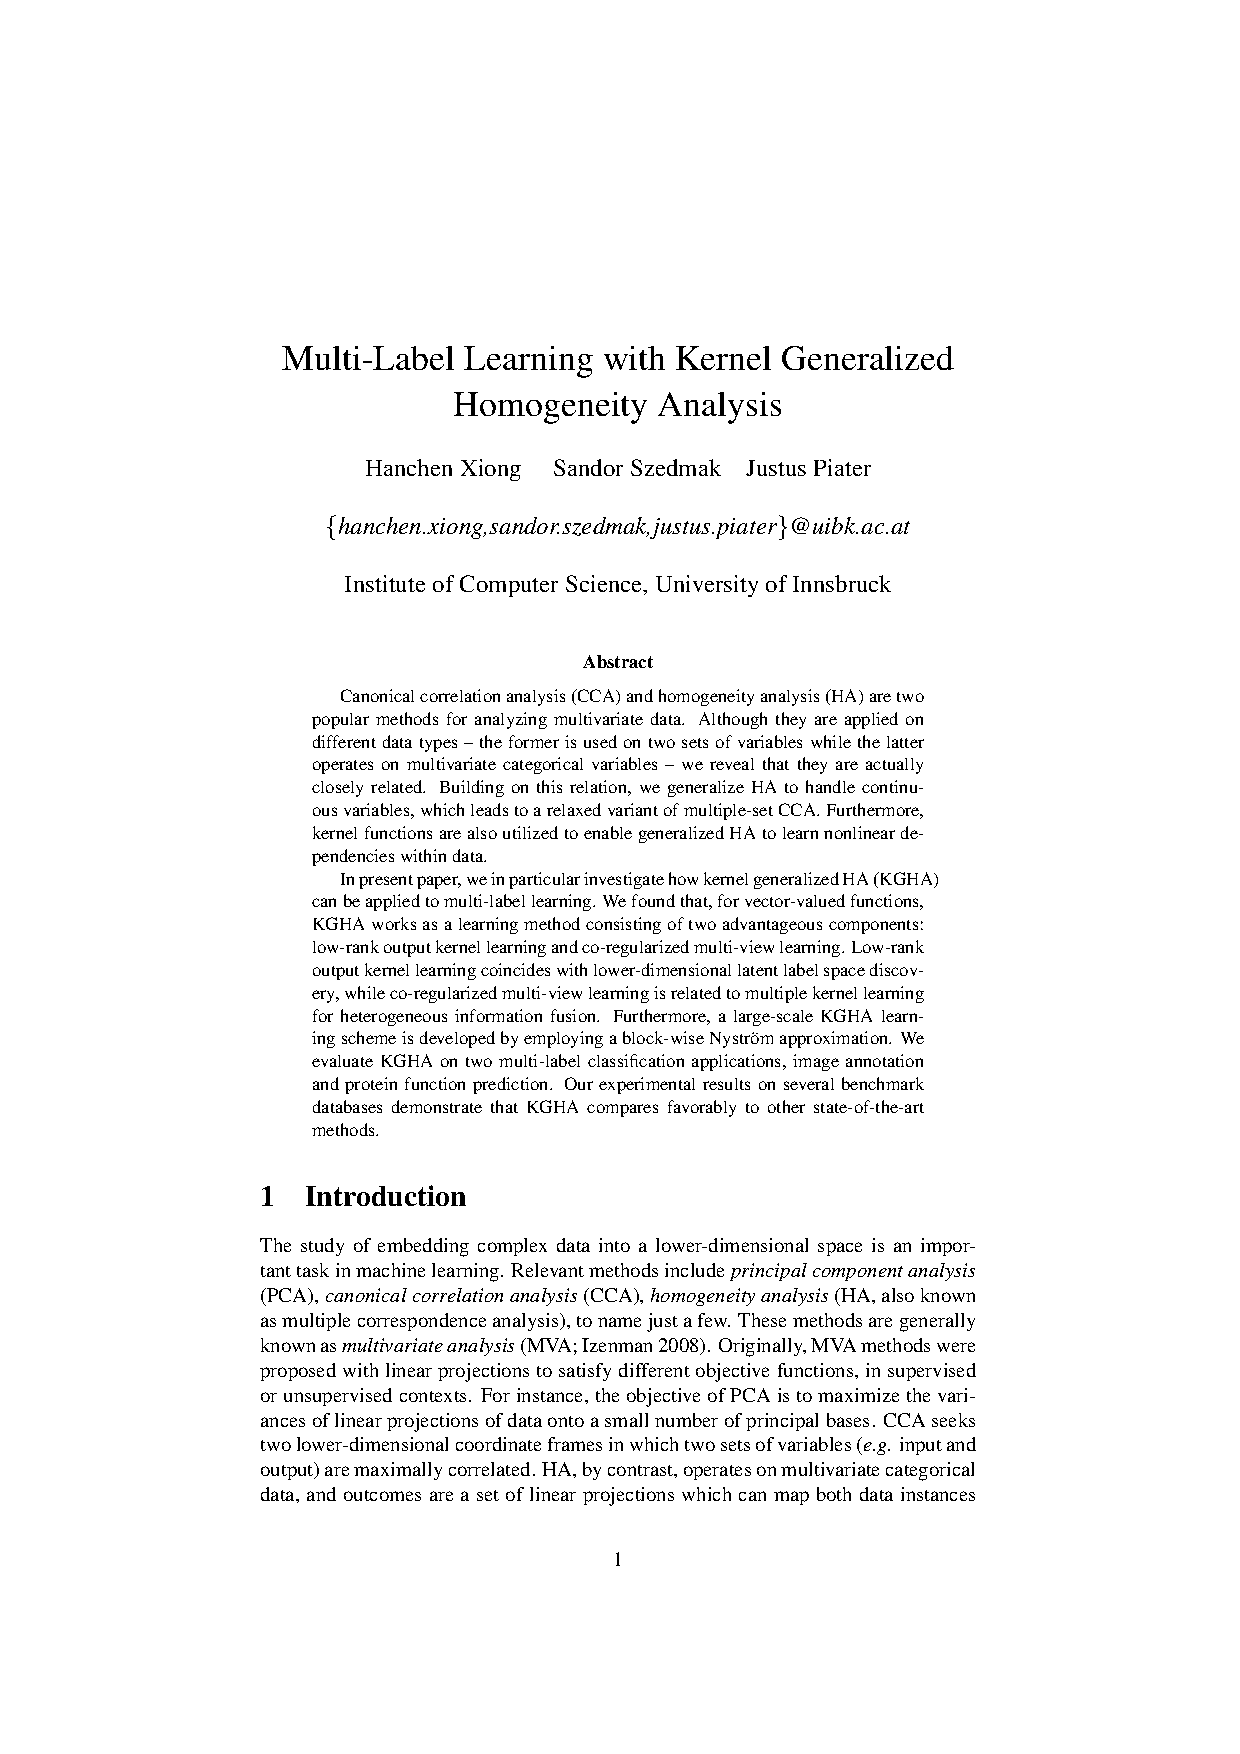
\includepdf[offset=3cm -3cm, scale=1.2, pages=-,pagecommand={\pagestyle{fancy}}]{./Papers/KGHA.pdf}

